% mpsub.tex -- Computational Optimization and Applications (COAP) format
% Document class: svjour3 (Springer format for COAP)
\RequirePackage{fix-cm}
\documentclass[smallextended]{svjour3}

\smartqed  % flush right qed marks, e.g. at end of proof

\journalname{Computational Optimization and Applications}

% Packages
\usepackage[T1]{fontenc}
\usepackage{amsmath}
\usepackage{amssymb}
\usepackage{amsfonts}
\usepackage{graphicx}
\usepackage{booktabs}
\usepackage{multirow}
\usepackage{algorithm}
\usepackage{algorithmic}
\usepackage{bm}
\usepackage{mathtools}
\usepackage{url}
\usepackage{marvosym}
\usepackage{hyperref}

% Theorem-like environments
\spdefaulttheorem{assumption}{Assumption}{\bfseries}{\itshape}

% Running headers
\titlerunning{MpSub: subspace trust-region derivative-free LLM fine-tuning}
\authorrunning{Y.~Wang, H.~Yao, and P.~Xie}

%%%%%%%%%%% Custom macros %%%%%%%%%%%
\newcommand{\bx}{\bm{x}}
\newcommand{\dd}{\bm{d}}
\newcommand{\B}{\bm{B}}
\newcommand{\bP}{\bm{P}}
\newcommand{\bd}{\bm{d}}
\newcommand{\bg}{\bm{g}}
\newcommand{\bz}{\bm{z}}
\newcommand{\bs}{\bm{s}}
\providecommand{\coloneqq}{\mathrel{\mathop:}=}
%%%%%%%%%%%

\begin{document}

\title{MpSub: A Momentum $p$-Dimensional Subspace Trust-Region Method for Derivative-Free Fine-Tuning of Large Language Models}

\author{Yuyang Wang \and Haoyu Yao \and Pengcheng Xie}

\institute{Y. Wang \and H. Yao \at
              Xi'an Jiaotong University, Xi'an, China \\
              \email{vibrancy05@stu.xjtu.edu.cn}, \email{yaohaoyu@stu.xjtu.edu.cn}
           \and
           P. Xie (\Letter) \at
              Lawrence Berkeley National Laboratory, Berkeley, CA, USA \\
              \email{pxie@lbl.gov}
}

\date{Received: date / Accepted: date}

\maketitle

\begin{abstract}
Zeroth-order optimization avoids the high activation memory of backpropagation in fine-tuning large language models, but existing methods rely on sensitive learning rates that require costly per-task tuning. We propose \texttt{MpSub}, a momentum $p$-dimensional subspace trust-region method. At each iteration, \texttt{MpSub} optimizes over a subspace combining the historical momentum of the last accepted step with random exploration directions. Subspace gradients are estimated via central differences, and trial steps are solved from a linear trust-region model. The trust-region radius adapts dynamically via an agreement ratio and governs both the finite-difference perturbation and step bounds, eliminating the need for a manual learning rate. Directions are regenerated in place from random seeds, maintaining $\mathcal{O}(n)$ auxiliary memory without storing the subspace basis. Under Gaussian direction sampling on smooth deterministic objectives, we bound the finite-difference error, quantify the gradient captured by the subspace, and establish almost-sure global convergence ($\liminf_{k\to\infty} \|\nabla f(\bx_k)\|_2 = 0$). On CommitmentBank under a matched budget of 8,400 forward passes, \texttt{MpSub} achieves mean test accuracies of 0.673 on OPT-125M and 0.690 on OPT-350M with fixed default parameters, matching MeZO tuned via extensive learning-rate search (0.685 at both sizes).

\keywords{Derivative-free optimization \and Subspace trust region \and Zeroth-order optimization \and Large language model fine-tuning}
\subclass{90C56 \and 65K05 \and 90C26}
\end{abstract}

\section{Introduction}
\label{sec:intro}

Zeroth-order (ZO) optimization has become an attractive alternative for full-parameter fine-tuning of large language models (LLMs) when backpropagation is limited by memory. Instead of storing activations for a backward pass, ZO methods estimate update directions from function evaluations. MeZO \cite{malladi2023mezo} applies the classical two-point random estimator \cite{nesterov2017random} to language models and regenerates random perturbations from seeds rather than storing them. Later methods have modified the perturbation structure, including random low-dimensional subspaces \cite{yu2024subzero} and low-rank gradient structures \cite{chen2024enhancing}.

These methods still use a prescribed learning rate to determine the update size. Its effective value can vary substantially across settings and may require a separate search. In addition, a single random direction contains only a small amount of directional information in a very high-dimensional parameter space. For a normalized isotropic direction, the typical magnitude of its projection onto a fixed gradient decreases as the dimension grows. This motivates using more than one search direction while avoiding a proportional increase in stored parameter-sized vectors.

Trust-region methods provide a natural way to control the step size without prescribing a learning rate. In derivative-free optimization, the trust-region radius is adjusted according to the agreement between a local model and the observed objective values \cite{audet2017derivative,conn2009introduction,conn2000trust,Conn2009a}. Direct model construction in the full parameter space is not practical for models with hundreds of millions of variables, which motivates restricting the search to a much smaller subspace \cite{cartis2023scalable,yuan2007subspace,yuan2014review}. Randomized subspaces have also been studied in derivative-free optimization \cite{cartis2024randomizedsubspacederivativefreeoptimization,kozak2021stochastic,Menickelly2023}.

The closest method to the present work is 2D-MoSub \cite{xie2023twodimensional}. It searches in a two-dimensional subspace formed by the previous accepted step and a new search direction. The previous step carries information from the optimization trajectory, while the new direction provides exploration. A quadratic interpolation model is constructed in this two-dimensional subspace and minimized within a trust region. This combination of momentum and random exploration is also the starting point of our method. The difficulty in extending the same approach to a larger subspace lies in the quadratic model: a direct extension to dimension $p$ would require $\frac{1}{2}(p+1)(p+2)$ interpolation points. At $p=20$, this would require 231 points before a trial step is computed.

We therefore consider the LLM fine-tuning problem
\begin{equation}
\min_{\bx \in \mathbb{R}^n}
\ \mathbb{E}_{\xi\sim\mathcal D}
\bigl[\ell(\bx;\xi)\bigr],
\label{eq:ft_objective}
\end{equation}
and propose \texttt{MpSub}, a momentum $p$-dimensional subspace trust-region method. \texttt{MpSub} preserves the momentum and exploration framework of 2D-MoSub but replaces quadratic interpolation with directional derivatives estimated by central differences. These estimates define a linear model in a $p$-dimensional subspace formed by the most recent accepted displacement and $p-1$ newly sampled Gaussian directions. The resulting iteration requires $2p+2$ function evaluations, so the evaluation cost grows linearly with the subspace dimension. For LLM fine-tuning, evaluations within each iteration share a fixed minibatch, and search directions are reconstructed dynamically from random seeds rather than stored explicitly.

For smooth deterministic objectives, we analyze the Gaussian directions directly without orthogonality assumptions. We derive finite-difference error bounds, quantify the gradient captured by the random subspace, and prove almost-sure global convergence ($\liminf_{k\to\infty} \|\nabla f(\bx_k)\|_2 = 0$) under a safeguarded trust-region radius update. We then compare \texttt{MpSub} with MeZO on OPT-125M and OPT-350M under matched forward-evaluation budgets.

\section{MpSub}
\label{section:MpSub}

We consider the unconstrained optimization problem
\begin{equation}
\min_{\bx \in \mathbb{R}^n}\ f(\bx),
\label{eq:opt_problem}
\end{equation}
in the regime where the parameter dimension $n$ is very large (e.g., $n \sim 10^8$ in full-parameter language model fine-tuning) and derivative information is inaccessible.

At each iteration $k$, \texttt{MpSub} maintains the parameter iterate $\bx_k \in \mathbb{R}^n$, a trust-region radius $\Delta_k \in [\Delta_{\min}, \Delta_{\max}]$, and a momentum displacement $\bm m_k \in \mathbb{R}^n$ from the most recent accepted step. The radius $\Delta_k$ serves as both the finite-difference perturbation scale and the trust-region bound. The overall procedure is summarized in Algorithm~\ref{alg:mpsub}.

\begin{algorithm}[htbp]
\caption{\texttt{MpSub}: momentum $p$-dimensional subspace trust-region method}
\label{alg:mpsub}
\begin{algorithmic}[1]
\STATE{\textbf{Input:} Initial iterate $\bx_0 \in \mathbb{R}^n$, subspace dimension $p \ge 2$, initial radius $\Delta_0 \in [\Delta_{\min}, \Delta_{\max}]$, parameters $0 < \gamma_1 < 1 < \gamma_2$, bounds $0 < \Delta_{\min} < \Delta_{\max}$, and threshold $\eta \in (0, 1)$.}
\STATE{Initialize momentum displacement $\bm{m}_0 = \bm{0}$.}
\FOR{$k = 0, 1, 2, \ldots$}
    \STATE{\textbf{1. Subspace generation:}}
    \STATE{\quad $\bd_1^{(k)} = \begin{cases} \bm{m}_k / \|\bm{m}_k\|_2, & \text{if } \|\bm{m}_k\|_2 > 0, \\ \bz_1 / \sqrt{n} \text{ with } \bz_1 \sim \mathcal{N}(\bm 0, \bm I_n), & \text{otherwise}. \end{cases}$}
    \STATE{\quad Sample $\bz_i \sim \mathcal{N}(\bm 0, \bm I_n)$ and set $\bd_i^{(k)} = \bz_i / \sqrt{n}$ independently for $i = 2, \ldots, p$.}
    \STATE{\textbf{2. Subspace gradient estimation:}}
    \STATE{\quad Compute directional derivatives for $i = 1, \ldots, p$ via central differences:}
    \STATE{\qquad $g_{k,i} = \frac{f(\bx_k + \Delta_k \bd_i^{(k)}) - f(\bx_k - \Delta_k \bd_i^{(k)})}{2\Delta_k}$, \quad and set $\bg_k = (g_{k,1}, \ldots, g_{k,p})^\top$.}
    \STATE{\textbf{3. Trust-region trial step:}}
    \STATE{\quad Compute coordinate step $\bs_s = -\Delta_k \bg_k / \|\bg_k\|_2$ and trial iterate $\bx^+ = \bx_k + \sum_{i=1}^p s_{s,i} \bd_i^{(k)}$.}
    \STATE{\quad Compute agreement ratio $\rho_k = \frac{f(\bx_k) - f(\bx^+)}{\Delta_k \|\bg_k\|_2}$.}
    \STATE{\textbf{4. Acceptance and radius update:}}
    \STATE{\quad \textbf{if} $f(\bx^+) < f(\bx_k)$ \textbf{then} $\bx_{k+1} = \bx^+$, $\bm{m}_{k+1} = \bx^+ - \bx_k$ \textbf{else} $\bx_{k+1} = \bx_k$, $\bm{m}_{k+1} = \bm{m}_k$.}
    \STATE{\quad \textbf{if} $\rho_k \geq \eta$ \textbf{then} $\Delta_{k+1} = \min\{\gamma_2 \Delta_k, \Delta_{\max}\}$ \textbf{else} $\Delta_{k+1} = \max\{\gamma_1 \Delta_k, \Delta_{\min}\}$.}
\ENDFOR
\end{algorithmic}
\end{algorithm}

\subsection{Subspace construction}
\label{subsec:construction}

At iteration $k$, optimization is restricted to the affine subspace $\bx_k + \mathcal{S}_k$, where $\mathcal{S}_k \subset \mathbb{R}^n$ is spanned by $p$ direction vectors $\bd_1^{(k)}, \ldots, \bd_p^{(k)}$. Gathering these directions as columns of the frame matrix $\bm D_k = [\bd_1^{(k)}, \ldots, \bd_p^{(k)}] \in \mathbb{R}^{n \times p}$, candidate displacements within $\mathcal{S}_k$ are parameterized by a coordinate vector $\bs_s \in \mathbb{R}^p$ via
\begin{equation}
\bx(\bs_s) = \bx_k + \bm D_k \bs_s = \bx_k + \sum_{i=1}^p s_{s,i} \bd_i^{(k)}.
\label{eq:subspace_param}
\end{equation}

The first search direction $\bd_1^{(k)}$ incorporates momentum from the optimization trajectory. When an accepted step is available, it is set to the normalized displacement
\begin{equation}
\bd_1^{(k)} = \frac{\bm m_k}{\|\bm m_k\|_2},
\label{eq:momentum_dir}
\end{equation}
where $\bm m_k$ denotes the parameter change resulting from the most recent successful step. Because consecutive descent steps in continuous optimization often exhibit directional correlation, retaining \eqref{eq:momentum_dir} incorporates directional information from previous successful steps into the subspace without requiring additional function evaluations. The remaining $p-1$ directions are drawn independently as
\begin{equation}
\bd_i^{(k)} = \frac{\bz_i}{\sqrt{n}}, \qquad \bz_i \sim \mathcal{N}(\bm{0}, \bm{I}_n), \quad i = 2, \ldots, p,
\label{eq:random_dirs}
\end{equation}
with the same distribution supplying $\bd_1^{(k)}$ when no accepted step is available. The factor $1/\sqrt{n}$ normalizes the expected squared Euclidean norm, $\mathbb E\|\bd_i^{(k)}\|_2^2 = 1$.

A fundamental geometric property of high-dimensional Gaussian vectors is their near-orthogonality: for $i \ne j$,
\begin{equation}
\mathbb E\bigl[\bd_i^{(k)\top} \bd_j^{(k)}\bigr] = 0
\qquad\text{and}\qquad
\mathbb E\bigl[ \bigl(\bd_i^{(k)\top} \bd_j^{(k)}\bigr)^2 \bigr] = \frac{1}{n}.
\label{eq:near_ortho}
\end{equation}
Consequently, the pairwise inner products have root-mean-square magnitude $n^{-1/2} \approx 10^{-4}$ at $n \sim 10^8$. The exploratory directions can therefore be used directly without orthogonalization, avoiding additional computation and memory overhead. The dimension $p$ controls how many directional derivatives enter the subspace model; its choice is examined empirically in Section~\ref{sec:experiments}.

\subsection{Subspace model and trial step}
\label{subsec:gradient}
\label{subsec:trial}

For each direction $\bd_i^{(k)}$, \texttt{MpSub} estimates the corresponding directional derivative via central differences:
\begin{equation}
g_{k,i} = \frac{f(\bx_k + \Delta_k \, \bd_i^{(k)}) - f(\bx_k - \Delta_k \, \bd_i^{(k)})}{2\Delta_k}, \quad i = 1, \ldots, p.
\label{eq:central_diff}
\end{equation}
The subspace gradient $\bg_k = (g_{k,1}, \ldots, g_{k,p})^\top \in \mathbb{R}^p$ collects these directional estimates, where each entry $g_{k,i}$ approximates $\nabla f(\bx_k)^\top \bd_i^{(k)}$. Setting the finite-difference perturbation to $\Delta_k$ directly links the sampling scale to the trust-region radius. Under the Lipschitz continuity of $\nabla f$, the finite-difference error is bounded linearly by $\Delta_k$ (Lemma~\ref{lem:fd}).

The estimated gradient defines a local linear surrogate model on the subspace coordinates:
\begin{equation}
m_k(\bs_s) = f(\bx_k) + \bg_k^\top \bs_s.
\label{eq:linear_model}
\end{equation}
The trial step is determined by minimizing this linear model subject to the trust-region constraint:
\begin{equation}
\min_{\bs_s \in \mathbb{R}^p}\; \bg_k^\top \bs_s \quad \text{subject to} \quad \|\bs_s\|_2 \leq \Delta_k.
\label{eq:subproblem_formulation}
\end{equation}
Whenever $\bg_k \ne \bm 0$, problem~\eqref{eq:subproblem_formulation} admits the unique closed-form solution
\begin{equation}
\bs_s = -\Delta_k \frac{\bg_k}{\|\bg_k\|_2},
\label{eq:closed_form_step}
\end{equation}
which corresponds to the steepest descent direction on the trust-region boundary. Mapping $\bs_s$ back to the ambient parameter space via \eqref{eq:subspace_param} yields the candidate iterate
\begin{equation}
\bx^+ = \bx_k + \bm D_k \bs_s = \bx_k - \frac{\Delta_k}{\|\bg_k\|_2} \sum_{i=1}^p g_{k,i} \bd_i^{(k)},
\label{eq:full_trial_point}
\end{equation}
with the predicted objective reduction given by
\begin{equation}
\operatorname{pred}_k = m_k(\bm 0) - m_k(\bs_s) = -\bg_k^\top \bs_s = \Delta_k \|\bg_k\|_2 > 0.
\label{eq:pred_reduction}
\end{equation}
If $\bg_k = \bm 0$, the estimated gradient vanishes across the subspace; in this event, the method contracts the trust-region radius, sets $\bx_{k+1} = \bx_k$ and $\bm m_{k+1} = \bm m_k$, and proceeds to the next iteration without evaluating an additional trial point.

\subsection{Acceptance and radius update}
\label{subsec:update}

Upon evaluating the candidate loss $f^+ = f(\bx^+)$, \texttt{MpSub} assesses the agreement between the surrogate model and the objective through the ratio
\begin{equation}
\rho_k = \frac{f(\bx_k) - f(\bx^+)}{\Delta_k \|\bg_k\|_2}.
\label{eq:agreement_ratio}
\end{equation}
The algorithm decouples iterate acceptance from trust-region radius adaptation (Step 4). The candidate point is accepted whenever it yields a strict objective decrease:
\begin{equation}
\begin{aligned}
\bx_{k+1} &=
\begin{cases}
\bx^+, & \text{if } f(\bx^+) < f(\bx_k), \\
\bx_k, & \text{otherwise},
\end{cases}
\\[4pt]
\bm m_{k+1} &=
\begin{cases}
\bx^+ - \bx_k, & \text{if } f(\bx^+) < f(\bx_k), \\
\bm m_k, & \text{otherwise},
\end{cases}
\end{aligned}
\label{eq:accept_rule}
\end{equation}
while the trust-region radius is updated according to the ratio test:
\begin{equation}
\Delta_{k+1} =
\begin{cases}
\min\{\gamma_2 \Delta_k, \Delta_{\max}\}, & \text{if } \rho_k \geq \eta, \\
\max\{\gamma_1 \Delta_k, \Delta_{\min}\}, & \text{if } \rho_k < \eta.
\end{cases}
\label{eq:radius_update_rule}
\end{equation}

Unlike classical trust-region methods \cite{conn2000trust} that accept trial points only when $\rho_k \ge \eta$, the rules \eqref{eq:accept_rule}--\eqref{eq:radius_update_rule} separate acceptance from radius adjustment. In zeroth-order settings where forward passes dominate execution time, enforcing $\rho_k \ge \eta$ for step acceptance would discard trial points that achieve objective reduction whenever $0 < f(\bx_k) - f(\bx^+) < \eta \operatorname{pred}_k$. Under \eqref{eq:accept_rule}, every candidate yielding a strictly lower observed loss is retained. At the same time, the ratio $\rho_k$ regulates the trust-region radius: the trust region expands when the linear surrogate reliably predicts the objective reduction ($\rho_k \ge \eta$), and contracts when nonlinearities or estimation errors dominate ($\rho_k < \eta$).

\subsection{Algorithmic realization for LLM fine-tuning}
\label{subsec:llm_realization}

While Algorithm~\ref{alg:mpsub} is stated for a generic objective $f$, applying it to full-parameter fine-tuning of large language models requires addressing two practical issues: minibatch stochasticity and the memory cost of storing $p$ search directions.

\subsubsection{Consistent minibatch evaluation}
In stochastic language model fine-tuning, the objective available at training step $k$ is defined by a sampled minibatch $\mathcal B_k \subset \mathcal D$:
\begin{equation}
f_k(\bx) = \frac{1}{|\mathcal B_k|} \sum_{\xi \in \mathcal B_k} \ell(\bx; \xi).
\label{eq:minibatch_loss}
\end{equation}
To prevent batch sampling noise from distorting the trust-region ratio, the minibatch $\mathcal B_k$ is held fixed throughout iteration $k$: the baseline loss $f_k(\bx_k)$, the $2p$ central-difference evaluations $f_k(\bx_k \pm \Delta_k \bd_i^{(k)})$, and the trial evaluation $f_k(\bx^+)$ are all computed on the same minibatch $\mathcal B_k$. Holding $\mathcal B_k$ constant ensures that the estimated subspace gradient $\bg_k$ and the agreement ratio
\begin{equation}
\rho_k = \frac{f_k(\bx_k) - f_k(\bx^+)}{\Delta_k \|\bg_k\|_2}
\label{eq:minibatch_rho}
\end{equation}
reflect local model fidelity on a fixed sample rather than minibatch variance.

Across iterations, a new minibatch $\mathcal B_{k+1}$ is drawn, while $\Delta_k$ and $\bm m_k$ carry over to the next step. Each iteration requires $2p + 2$ forward passes on the training objective ($42$ passes when $p = 20$).

\subsubsection{In-place perturbations and seed regeneration}
Storing the frame matrix $\bm D_k \in \mathbb{R}^{n \times p}$ explicitly would require $pn$ floating-point numbers. For an LLM such as OPT-125M ($n \approx 1.25 \times 10^8$) with $p = 20$ in FP32, this would require approximately $10$~GB of memory, which exceeds the parameter storage of the model itself.

To avoid this memory overhead, \texttt{MpSub} never stores the matrix $\bm D_k$ explicitly in memory. Instead, each exploratory direction $\bd_i^{(k)}$ ($i = 2, \ldots, p$) is generated dynamically on the fly using a pseudorandom number generator reseeded deterministically by the iteration and direction indices. Weights are perturbed, evaluated, and restored in place, reconstructing directions as needed without storing them.

Once the subspace gradient $\bg_k$ and the coordinate step $\bs_s = -\Delta_k \bg_k / \|\bg_k\|_2$ are computed, the directions are regenerated a final time and combined in place to form the trial displacement
\begin{equation}
\bm u_k = \sum_{i=1}^p s_{s,i} \bd_i^{(k)}.
\label{eq:trial_displacement}
\end{equation}
The trial displacement $\bm u_k$ is formed directly in place while advancing the model weights to $\bx^+ = \bx_k + \bm u_k$. If the trial step is accepted, $\bm u_k$ is preserved as the new momentum displacement $\bm m_{k+1}$; if rejected, the base weights $\bx_k$ are immediately restored by subtracting $\bm u_k$.

Training is thus executed through forward inference passes alone. Auxiliary storage is limited to $\mathcal{O}(n)$ vectors for momentum and trial updates, keeping the training memory footprint at the inference level and independent of the subspace dimension $p$.

\section{Theoretical Analysis}
\label{sec:analysis}

We analyze \texttt{MpSub} for a deterministic objective under the Gaussian direction sampling used in Algorithm~\ref{alg:mpsub}. No orthogonality between the search directions is assumed. The analysis first gives error and descent bounds for a general frame $\bm D_k$, and then uses the distribution of the Gaussian directions to obtain a global first-order convergence result.

Throughout this section, we set $\Delta_{\min}=0$ for the asymptotic analysis. We also use the following safeguarded radius update with a fixed constant $\kappa>0$:
\begin{equation}
\label{eq:safeguarded_radius}
\Delta_{k+1} =
\begin{cases}
\min\{\gamma_2\Delta_k,\Delta_{\max}\}, & \text{if } \rho_k\ge\eta \text{ and } \|\bg_k\|_2\ge\kappa\Delta_k, \\
\gamma_1\Delta_k, & \text{otherwise}.
\end{cases}
\end{equation}
As in Algorithm~\ref{alg:mpsub}, a trial step is accepted whenever $f(\bx^+) < f(\bx_k)$.

\begin{assumption}
\label{ass:smooth}
The objective function $f:\mathbb R^n\to\mathbb R$ is continuously differentiable and bounded below. Its gradient is Lipschitz continuous with constant $L>0$:
\begin{equation}
\label{eq:lipschitz_grad}
\|\nabla f(\bx)-\nabla f(\bm y)\|_2 \le L\|\bx-\bm y\|_2, \qquad \forall\, \bx,\bm y\in\mathbb R^n.
\end{equation}
\end{assumption}

Let $\bm D_k = [\bd_1^{(k)},\ldots,\bd_p^{(k)}] \in \mathbb{R}^{n \times p}$ be the frame generated at iteration $k$, and define the exact directional derivatives
\[
\hat g_{k,i} \coloneqq \nabla f(\bx_k)^\top\bd_i^{(k)}, \qquad \hat{\bg}_k \coloneqq \bm D_k^\top\nabla f(\bx_k).
\]
The finite-difference estimates are denoted by
\[
\bg_k = (g_{k,1},\ldots,g_{k,p})^\top, \qquad g_{k,i} = \frac{f(\bx_k+\Delta_k\bd_i^{(k)}) - f(\bx_k-\Delta_k\bd_i^{(k)})}{2\Delta_k}.
\]

\subsection{Finite differences and random subspaces}
\label{subsec:estimation}

We first bound the finite-difference error without assuming that the directions have unit norm.

\begin{lemma}[Finite-difference error]
\label{lem:fd_general}
\label{lem:fd}
Suppose Assumption~\ref{ass:smooth} holds. Then
\begin{equation}
\label{eq:fd_general_component}
|g_{k,i}-\hat g_{k,i}| \le \frac{L\Delta_k}{2} \|\bd_i^{(k)}\|_2^2, \qquad i=1,\ldots,p.
\end{equation}
Consequently,
\begin{equation}
\label{eq:fd_general_vector}
\|\bg_k-\hat{\bg}_k\|_2 \le \frac{L\Delta_k}{2} Q_k, \qquad Q_k \coloneqq \left( \sum_{i=1}^p \|\bd_i^{(k)}\|_2^4 \right)^{1/2}.
\end{equation}
\end{lemma}

\begin{proof}
For any direction $\bd$ and $t>0$, Lipschitz continuity of the gradient gives
\[
\left| f(\bx_k+t\bd) - f(\bx_k) - t\nabla f(\bx_k)^\top\bd \right| \le \frac{L}{2}t^2\|\bd\|_2^2.
\]
Applying this bound to $t=\Delta_k$ in the directions $\bd_i^{(k)}$ and $-\bd_i^{(k)}$, write
\[
f(\bx_k+\Delta_k\bd_i^{(k)}) = f(\bx_k) + \Delta_k\hat g_{k,i} + R_{i,+},
\]
and
\[
f(\bx_k-\Delta_k\bd_i^{(k)}) = f(\bx_k) - \Delta_k\hat g_{k,i} + R_{i,-},
\]
where $|R_{i,\pm}| \le \frac{L\Delta_k^2}{2} \|\bd_i^{(k)}\|_2^2$.
Subtracting the two expressions gives
\[
g_{k,i}-\hat g_{k,i} = \frac{R_{i,+}-R_{i,-}}{2\Delta_k},
\]
which proves \eqref{eq:fd_general_component}. Summing the squared componentwise bounds gives \eqref{eq:fd_general_vector}.
\qed
\end{proof}
We now analyze the gradient captured by the Gaussian directions in Algorithm~\ref{alg:mpsub}. Let $\mathcal F_k$ contain the algorithmic history before the random exploratory directions at iteration $k$ are sampled. Conditionally on $\mathcal F_k$,
\[
\bd_i^{(k)} = \frac{\bz_i}{\sqrt n}, \qquad \bz_i\sim\mathcal N(\bm0,\bm I_n), \qquad i=2,\ldots,p,
\]
independently.

\begin{lemma}[Gaussian gradient capture]
\label{lem:gaussian_capture}
\label{lem:capture}
Suppose $p\ge 2$, and let $\bm v_k = \nabla f(\bx_k)$. Conditionally on $\mathcal F_k$,
\begin{equation}
\label{eq:chi_square_capture}
\sum_{i=2}^p \left( \bm v_k^\top\bd_i^{(k)} \right)^2 \overset{d}{=} \frac{\|\bm v_k\|_2^2}{n} \chi^2_{p-1}.
\end{equation}
In particular,
\begin{equation}
\label{eq:expected_gaussian_capture}
\mathbb E \left[ \sum_{i=2}^p \left( \bm v_k^\top\bd_i^{(k)} \right)^2 \;\middle|\; \mathcal F_k \right] = \frac{p-1}{n} \|\bm v_k\|_2^2.
\end{equation}
Moreover, for every $q\in(0,1)$, there exist constants $\alpha>0$ and $R>1$, independent of $k$, such that whenever $\bm v_k\ne\bm 0$,
\begin{equation}
\label{eq:good_frame_probability}
\mathbb P \left( \|\hat{\bg}_k\|_2 \ge \alpha\|\bm v_k\|_2, \quad \max_{1\le i\le p} \|\bd_i^{(k)}\|_2 \le R \;\middle|\; \mathcal F_k \right) \ge q.
\end{equation}
\end{lemma}

\begin{proof}
For every $i=2,\ldots,p$,
\[
\bm v_k^\top\bd_i^{(k)} = \frac{\bm v_k^\top\bz_i}{\sqrt n} \sim \mathcal N \left( 0, \frac{\|\bm v_k\|_2^2}{n} \right),
\]
and these random variables are conditionally independent. Equation~\eqref{eq:chi_square_capture} follows immediately, and taking expectations gives \eqref{eq:expected_gaussian_capture}.

To prove \eqref{eq:good_frame_probability}, fix $q\in(0,1)$. Since $p\ge 2$, a $\chi^2_{p-1}$ random variable is positive almost surely. We can choose $\tau>0$ such that $\mathbb P(\chi^2_{p-1}\ge\tau) \ge 1 - \frac{1-q}{2}$. Setting $\alpha=\sqrt{\tau/n}$, equation~\eqref{eq:chi_square_capture} and $\|\hat{\bg}_k\|_2^2 \ge \sum_{i=2}^p (\bm v_k^\top\bd_i^{(k)})^2$ imply
\[
\mathbb P\left( \|\hat{\bg}_k\|_2 \ge \alpha\|\bm v_k\|_2 \;\middle|\; \mathcal F_k \right) \ge 1 - \frac{1-q}{2}.
\]
Similarly, since each $\|\bz_i\|_2/\sqrt n$ is almost surely finite and $\|\bd_1^{(k)}\|_2 \le 1$, we can choose $R>1$ such that $\mathbb P(\max_{1\le i\le p}\|\bd_i^{(k)}\|_2 \le R \mid \mathcal F_k) \ge 1 - \frac{1-q}{2}$. A union bound then gives \eqref{eq:good_frame_probability}.
\qed
\end{proof}

The next proposition bounds the objective decrease produced by the trial step for a general frame.

\begin{proposition}[Decrease for a general frame]
\label{prop:general_descent}
\label{prop:descent}
Suppose Assumption~\ref{ass:smooth} holds and $\bg_k\ne\bm0$. Let
\[
\bs_k = -\Delta_k \frac{\bg_k}{\|\bg_k\|_2}, \qquad \bx_k^+ = \bx_k+\bm D_k\bs_k,
\]
and define $\beta_k \coloneqq \|\bm D_k\|_2$. Then
\begin{equation}
\label{eq:general_decrease}
f(\bx_k)-f(\bx_k^+) \ge \Delta_k\|\bg_k\|_2 - \frac{L\Delta_k^2}{2} (Q_k+\beta_k^2).
\end{equation}
Consequently,
\begin{equation}
\label{eq:general_ratio}
\rho_k \ge 1 - \frac{L\Delta_k(Q_k+\beta_k^2)}{2\|\bg_k\|_2}.
\end{equation}
\end{proposition}

\begin{proof}
Let $\bm h_k = \bm D_k\bs_k$. Since $\hat{\bg}_k = \bm D_k^\top\nabla f(\bx_k)$, we have $\nabla f(\bx_k)^\top\bm h_k = \hat{\bg}_k^\top\bs_k$. Using $\bg_k^\top\bs_k = -\Delta_k\|\bg_k\|_2$ and Lemma~\ref{lem:fd_general},
\[
\begin{aligned}
\nabla f(\bx_k)^\top\bm h_k &= \bg_k^\top\bs_k + (\hat{\bg}_k-\bg_k)^\top\bs_k \\
&\le -\Delta_k\|\bg_k\|_2 + \|\hat{\bg}_k-\bg_k\|_2\|\bs_k\|_2 \\
&\le -\Delta_k\|\bg_k\|_2 + \frac{LQ_k}{2}\Delta_k^2.
\end{aligned}
\]
Also, $\|\bm h_k\|_2 \le \|\bm D_k\|_2\|\bs_k\|_2 = \beta_k\Delta_k$. The descent lemma therefore gives
\[
\begin{aligned}
f(\bx_k^+) &\le f(\bx_k) + \nabla f(\bx_k)^\top\bm h_k + \frac{L}{2}\|\bm h_k\|_2^2 \\
&\le f(\bx_k) - \Delta_k\|\bg_k\|_2 + \frac{L\Delta_k^2}{2} (Q_k+\beta_k^2),
\end{aligned}
\]
which proves \eqref{eq:general_decrease}. Dividing by the predicted reduction $\Delta_k\|\bg_k\|_2$ gives \eqref{eq:general_ratio}.
\qed
\end{proof}

\subsection{Global convergence}
\label{subsec:global_convergence}

We first show that the squared trust-region radii are summable. Let
\begin{equation}
\label{eq:expansion_set}
\mathcal S \coloneqq \left\{ k : \rho_k\ge\eta \text{ and } \|\bg_k\|_2\ge\kappa\Delta_k \right\}
\end{equation}
denote the set of iterations at which the trust-region radius is expanded.

\begin{lemma}[Summability of the trust-region radii]
\label{lem:radius_summability}
\label{lem:radius_decay}
Suppose Assumption~\ref{ass:smooth} holds, $\Delta_{\min}=0$, and the radius is updated according to \eqref{eq:safeguarded_radius}. Then
\begin{equation}
\label{eq:radius_square_summable}
\sum_{k=0}^{\infty}\Delta_k^2 < \infty.
\end{equation}
In particular,
\begin{equation}
\label{eq:radius_to_zero}
\lim_{k\to\infty} \Delta_k = 0.
\end{equation}
\end{lemma}

\begin{proof}
For any $k \in \mathcal S$, the definition of $\rho_k$ and \eqref{eq:expansion_set} give
\[
f(\bx_k)-f(\bx_k^+) = \rho_k\Delta_k\|\bg_k\|_2 \ge \eta\kappa\Delta_k^2.
\]
Since the right-hand side is strictly positive, the trial point is accepted. Because $f$ is bounded below by a finite constant $f_{\mathrm{low}}$, summing over all successful expansion steps yields
\[
\sum_{k\in\mathcal S}\Delta_k^2 \le \frac{f(\bx_0)-f_{\mathrm{low}}}{\eta\kappa} < \infty.
\]
For every iteration $k$, the update rule \eqref{eq:safeguarded_radius} implies
\[
\Delta_{k+1}^2 \le \gamma_1^2\Delta_k^2 + \gamma_2^2\Delta_k^2\mathbf{1}_{\{k\in\mathcal S\}}.
\]
Summing this inequality from $k=0$ to $N$ yields
\[
(1-\gamma_1^2) \sum_{k=1}^{N}\Delta_k^2 + \Delta_{N+1}^2 \le \gamma_1^2\Delta_0^2 + \gamma_2^2 \sum_{k\in\mathcal S}\Delta_k^2.
\]
Because $\gamma_1\in(0,1)$, we have $1-\gamma_1^2 > 0$. Taking $N\to\infty$ establishes \eqref{eq:radius_square_summable}, which directly implies $\lim_{k\to\infty}\Delta_k = 0$.
\qed
\end{proof}

This leads to subsequential convergence of the gradient norm.

\begin{theorem}[Subsequential convergence]
\label{thm:liminf_convergence}
Suppose Assumption~\ref{ass:smooth} holds and $p\ge2$. Let the exploratory directions be sampled independently as
\[
\bd_i^{(k)} = \frac{\bz_i}{\sqrt n}, \qquad \bz_i\sim\mathcal N(\bm0,\bm I_n), \qquad i=2,\ldots,p.
\]
Then
\begin{equation}
\label{eq:liminf_gradient}
\liminf_{k\to\infty} \|\nabla f(\bx_k)\|_2 = 0 \qquad \text{almost surely}.
\end{equation}
\end{theorem}

\begin{proof}
Suppose, to the contrary, that there exist $\varepsilon>0$ and an index $K_0$ such that
\begin{equation}
\label{eq:gradient_lower_contradiction}
\|\nabla f(\bx_k)\|_2 \ge \varepsilon, \qquad \forall\, k\ge K_0.
\end{equation}
Choose a probability threshold
\begin{equation}
\label{eq:q_condition}
q > \max\left\{ \frac{1}{2},\, \frac{\log(1/\gamma_1)}{\log(\gamma_2/\gamma_1)} \right\}.
\end{equation}
By Lemma~\ref{lem:gaussian_capture}, there exist constants $\alpha>0$ and $R>1$ such that the event
\[
G_k \coloneqq \left\{ \|\hat{\bg}_k\|_2 \ge \alpha\|\nabla f(\bx_k)\|_2, \quad \max_{1\le i\le p}\|\bd_i^{(k)}\|_2\le R \right\}
\]
satisfies $\mathbb P(G_k\mid\mathcal F_k)\ge q$. On $G_k$, we have $Q_k\le\sqrt p\,R^2$ and $\|\bm D_k\|_2^2\le pR^2$. Applying Lemma~\ref{lem:fd_general} under \eqref{eq:gradient_lower_contradiction} gives
\[
\|\bg_k\|_2 \ge \|\hat{\bg}_k\|_2 - \|\bg_k-\hat{\bg}_k\|_2 \ge \alpha\varepsilon - \frac{L\sqrt p\,R^2}{2}\Delta_k.
\]
Since $\Delta_k\to0$ by Lemma~\ref{lem:radius_summability}, for all sufficiently large $k$ we have $\gamma_2\Delta_k \le \Delta_{\max}$ and
\begin{equation}
\label{eq:g_lower_good}
\|\bg_k\|_2 \ge \frac{\alpha\varepsilon}{2}.
\end{equation}
Proposition~\ref{prop:general_descent} then ensures that, on $G_k$ and for all sufficiently large $k$,
\[
\rho_k\ge\eta \qquad \text{and} \qquad \|\bg_k\|_2\ge\kappa\Delta_k.
\]
Because $\gamma_2\Delta_k \le \Delta_{\max}$ holds for all large $k$, the update rule \eqref{eq:safeguarded_radius} on $G_k$ produces $\Delta_{k+1}=\gamma_2\Delta_k$ without truncation, while on the remaining iterations $\Delta_{k+1}\ge\gamma_1\Delta_k$.

Let $I_k \coloneqq \mathbf{1}_{G_k}$. For all sufficiently large $k$,
\begin{equation}
\label{eq:log_radius_increment}
\log\Delta_{k+1}-\log\Delta_k \ge I_k\log\gamma_2 + (1-I_k)\log\gamma_1.
\end{equation}
Since $\mathbb E[I_k\mid\mathcal F_k] \ge q$, the strong law of large numbers for bounded martingale differences implies
\[
\liminf_{N\to\infty} \frac{1}{N} \sum_{k=K}^{K+N-1} I_k \ge q \qquad \text{almost surely}.
\]
Averaging \eqref{eq:log_radius_increment} over $N$ steps therefore yields
\[
\liminf_{N\to\infty} \frac{\log\Delta_{K+N}-\log\Delta_K}{N} \ge q\log\gamma_2 + (1-q)\log\gamma_1 > 0 \qquad \text{almost surely},
\]
where the strict inequality follows from \eqref{eq:q_condition}. This implies $\Delta_k \to \infty$, contradicting $\Delta_k\to0$ from Lemma~\ref{lem:radius_summability}. Thus \eqref{eq:gradient_lower_contradiction} cannot hold, establishing \eqref{eq:liminf_gradient}.
\qed
\end{proof}

Theorem~\ref{thm:liminf_convergence} establishes almost-sure subsequential convergence, consistent with standard first-order guarantees in derivative-free trust-region optimization \cite{conn2009introduction,conn2000trust}.

To examine under what conditions the entire sequence of gradient norms converges to zero, fix any $\varepsilon>0$ and define the index set of large gradients:
\begin{equation}
\mathcal K_\varepsilon \coloneqq \left\{ k : \|\nabla f(\bx_k)\|_2 > \varepsilon \right\}.
\end{equation}

\begin{lemma}
\label{lem:radius_sum_large_gradient}
Under the assumptions of Theorem~\ref{thm:liminf_convergence}, for every $\varepsilon>0$,
\begin{equation}
\label{eq:good_frame_sum}
\sum_{k\in\mathcal K_\varepsilon\cap G_k}\Delta_k < \infty \qquad \text{almost surely}.
\end{equation}
If, additionally, the renewal property for probabilistically accurate models holds along $\mathcal K_\varepsilon$ \cite{bandeira2014convergence,Gratton-2017} (that is, the run length of consecutive unsuccessful iterations between occurrences of $G_k$ is stochastically dominated by a geometric distribution), then
\begin{equation}
\label{eq:radius_sum_large_gradient}
\sum_{k\in\mathcal K_\varepsilon}\Delta_k < \infty \qquad \text{almost surely}.
\end{equation}
\end{lemma}

\begin{proof}
Choose the good-frame event $G_k$ as in the proof of Theorem~\ref{thm:liminf_convergence} with conditional probability $q > 1/2$. Because $\Delta_k\to0$, whenever $k\in\mathcal K_\varepsilon\cap G_k$ and $k$ is sufficiently large, we have $\|\bg_k\|_2 \ge \frac{\alpha\varepsilon}{2}$ and $\rho_k\ge\eta$. Consequently,
\[
f(\bx_k)-f(\bx_{k+1}) \ge \frac{\eta\alpha\varepsilon}{2}\Delta_k.
\]
Because $f$ is bounded below, summing this decrease over all such iterations establishes \eqref{eq:good_frame_sum}. Under the renewal property, the total sum of radii over $\mathcal K_\varepsilon$ is bounded by a constant multiple of the sum over $\mathcal K_\varepsilon \cap G_k$, yielding \eqref{eq:radius_sum_large_gradient}.
\qed
\end{proof}

Recall that $\beta_k = \|\bm D_k\|_2$. Since the spectral norm is bounded by the Frobenius norm, we have
\[
\mathbb E[\beta_k^2\mid\mathcal F_k] \le \mathbb E\bigl[\|\bm D_k\|_{\mathrm{F}}^2 \;\big|\; \mathcal F_k\bigr] = \|\bd_1^{(k)}\|_2^2 + \sum_{i=2}^p \mathbb E\left[\frac{\|\bz_i\|_2^2}{n}\right] \le 1 + (p-1) = p,
\]
which implies $\sup_k \mathbb E[\beta_k^2\mid\mathcal F_k] \le p < \infty$. Because $\Delta_k$ is measurable with respect to $\mathcal F_k$, taking total expectations yields $\sum_{k=0}^{\infty} \mathbb E[\beta_k^2 \Delta_k^2] \le p \sum_{k=0}^{\infty} \mathbb E[\Delta_k^2] < \infty$ by Lemma~\ref{lem:radius_summability}, which guarantees $\sum_{k=0}^{\infty} \beta_k^2 \Delta_k^2 < \infty$ almost surely. In particular,
\begin{equation}
\label{eq:actual_step_decay}
\lim_{k\to\infty} \beta_k\Delta_k = 0 \qquad \text{almost surely},
\end{equation}
and, whenever \eqref{eq:radius_sum_large_gradient} holds,
\begin{equation}
\label{eq:actual_step_sum}
\sum_{k\in\mathcal K_\varepsilon} \beta_k\Delta_k < \infty \qquad \text{almost surely}.
\end{equation}

\begin{theorem}[Full global convergence]
\label{thm:global_convergence}
Under the assumptions of Theorem~\ref{thm:liminf_convergence}, if \eqref{eq:radius_sum_large_gradient} holds for every $\varepsilon>0$, then
\begin{equation}
\label{eq:gradient_convergence}
\lim_{k\to\infty} \|\nabla f(\bx_k)\|_2 = 0 \qquad \text{almost surely}.
\end{equation}
\end{theorem}

\begin{proof}
Suppose, for contradiction, that \eqref{eq:gradient_convergence} does not hold. In view of Theorem~\ref{thm:liminf_convergence}, there then exists $\varepsilon>0$ and infinitely many disjoint pairs of indices $a_j < b_j$ such that
\[
\|\nabla f(\bx_{a_j})\|_2 \le \varepsilon, \qquad \|\nabla f(\bx_{b_j})\|_2 > 2\varepsilon,
\]
while
\[
\|\nabla f(\bx_k)\|_2 > \varepsilon, \qquad \forall\, a_j < k < b_j.
\]
By the Lipschitz continuity of the gradient (Assumption~\ref{ass:smooth}),
\[
\varepsilon < \|\nabla f(\bx_{b_j})\|_2 - \|\nabla f(\bx_{a_j})\|_2 \le L \sum_{k=a_j}^{b_j-1} \|\bx_{k+1}-\bx_k\|_2.
\]
Since $\|\bx_{k+1}-\bx_k\|_2 \le \|\bm D_k \bs_k\|_2 \le \beta_k\Delta_k$, we can partition the summation as
\[
\sum_{k=a_j}^{b_j-1} \|\bx_{k+1}-\bx_k\|_2 \le \beta_{a_j}\Delta_{a_j} + \sum_{k=a_j+1}^{b_j-1} \beta_k\Delta_k.
\]
As $j\to\infty$, the first term $\beta_{a_j}\Delta_{a_j} \to 0$ almost surely by \eqref{eq:actual_step_decay}. Furthermore, all intermediate indices $k \in \{a_j+1, \ldots, b_j-1\}$ belong to $\mathcal K_\varepsilon$. Because $\sum_{k\in\mathcal K_\varepsilon} \beta_k\Delta_k < \infty$ almost surely by \eqref{eq:actual_step_sum}, the tail sum $\sum_{k=a_j+1}^{b_j-1} \beta_k\Delta_k$ tends to zero as $j\to\infty$. Consequently, the entire right-hand side converges to zero, which contradicts the strict lower bound $\varepsilon > 0$.

Therefore, \eqref{eq:gradient_convergence} holds almost surely.
\qed
\end{proof}

\section{Numerical Experiments}
\label{sec:experiments}

We evaluate \texttt{MpSub} on full-parameter fine-tuning of causal language models, comparing against the zeroth-order optimizer MeZO \cite{malladi2023mezo} under matched computational budgets. We also examine step-size sensitivity and the effect of the subspace dimension.

\subsection{Experimental setup}
\label{subsec:setup}

Experiments are conducted on CommitmentBank (CB) from the SuperGLUE benchmark, a three-class natural language inference task. Following \cite{malladi2023mezo}, we sample 100 training examples, reserve 50 examples for development, and evaluate on the standard 56-example validation split as the test set. We evaluate two autoregressive models from the OPT family: OPT-125M ($n \approx 1.25 \times 10^8$ parameters) and OPT-350M ($n \approx 3.5 \times 10^8$ parameters). All parameters are stored and optimized in FP32 with a batch size of 8. Results are averaged over three random seeds, with min--max ranges reported.

Because zeroth-order methods do not compute gradients, computational cost is measured by the total number of forward passes on the training objective. Each method is allotted a budget of $8{,}400$ training-objective forward passes (excluding periodic evaluations on the development set). For \texttt{MpSub} with $p = 20$, which takes 200 optimization steps, each iteration requires $2p + 2 = 42$ evaluations. MeZO uses 2 evaluations per step, thus executing $4{,}200$ steps.

\texttt{MpSub} uses the same fixed hyperparameters across both models: $p = 20$, initial radius $\Delta_0 = 10^{-1}$, contraction factor $\gamma_1 = 0.5$, expansion factor $\gamma_2 = 2.0$, success threshold $\eta = 0.1$, $\Delta_{\min} = 10^{-12}$, and $\Delta_{\max} = 1.0$. For MeZO, the perturbation scale is $\epsilon = 10^{-3}$, and the learning rate $\eta_{\mathrm{M}}$ is selected by development accuracy over a grid: $\{10^{-8}, 10^{-7}, 10^{-6}, 10^{-5}, 10^{-4}\}$ on OPT-125M and $\{10^{-7}, 10^{-6}, 10^{-5}\}$ on OPT-350M.

\subsection{Matched-budget comparison}
\label{subsec:main}

Table~\ref{tab:main} reports test and development accuracy across three random seeds under the common budget of $8{,}400$ forward passes.

\begin{table}[htb]
\centering
\caption{Matched-budget fine-tuning results on CommitmentBank ($8{,}400$ forward passes). Values are means over three random seeds, with min--max ranges in parentheses. The MeZO learning rate is selected by mean development accuracy.}
\label{tab:main}
\small
\begin{tabular}{@{}llccc@{}}
\toprule
Model & Method & Dev loss & Dev acc. & Test acc. \\
\midrule
OPT-125M & \texttt{MpSub} ($\Delta_0=10^{-1}$) & \shortstack{$0.674$ \\ {\scriptsize($0.620$--$0.723$)}} & \shortstack{$0.773$ \\ {\scriptsize($0.740$--$0.820$)}} & \shortstack{$0.673$ \\ {\scriptsize($0.661$--$0.679$)}} \\
         & MeZO ($\eta_{\mathrm M}=10^{-6}$) & \shortstack{$0.703$ \\ {\scriptsize($0.625$--$0.784$)}} & \shortstack{$0.760$ \\ {\scriptsize($0.740$--$0.800$)}} & \shortstack{$0.685$ \\ {\scriptsize($0.679$--$0.696$)}} \\
\midrule
OPT-350M & \texttt{MpSub} ($\Delta_0=10^{-1}$) & \shortstack{$0.738$ \\ {\scriptsize($0.715$--$0.774$)}} & \shortstack{$0.787$ \\ {\scriptsize($0.760$--$0.820$)}} & \shortstack{$0.690$ \\ {\scriptsize($0.679$--$0.714$)}} \\
         & MeZO ($\eta_{\mathrm M}=10^{-6}$) & \shortstack{$0.679$ \\ {\scriptsize($0.582$--$0.743$)}} & \shortstack{$0.780$ \\ {\scriptsize($0.720$--$0.880$)}} & \shortstack{$0.685$ \\ {\scriptsize($0.679$--$0.696$)}} \\
\bottomrule
\end{tabular}
\end{table}

On OPT-125M, \texttt{MpSub} with the default radius $\Delta_0 = 10^{-1}$ achieves a mean development accuracy of $0.773$ and a development loss of $0.674$, compared to $0.760$ and $0.703$ for MeZO, while test accuracies are similar ($0.673$ versus $0.685$). On OPT-350M, \texttt{MpSub} achieves a mean test accuracy of $0.690$ and development accuracy of $0.787$, compared to $0.685$ and $0.780$ for MeZO.

\begin{figure}[htb]
\centering
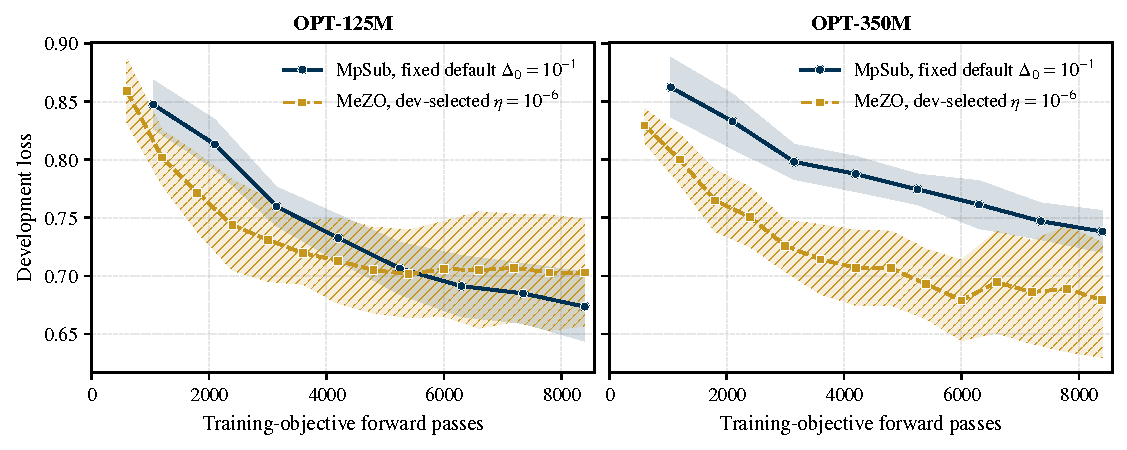
\includegraphics[width=0.98\textwidth]{fig_convergence_models.pdf}
\caption{Development loss versus training forward passes for OPT-125M (left) and OPT-350M (right). Shaded bands represent $\pm 1$ standard error of the mean across three random seeds.}
\label{fig:convergence}
\end{figure}

Figure~\ref{fig:convergence} shows development loss across forward passes. On OPT-125M, MeZO decreases quickly initially but then plateaus, whereas \texttt{MpSub} descends steadily to a lower final loss ($0.674$ vs.\ $0.703$). On OPT-350M, MeZO achieves a lower loss during training, but both methods reach similar final test accuracy ($0.690$ for \texttt{MpSub} vs.\ $0.685$ for MeZO).

\subsection{Step-size sensitivity}
\label{subsec:sensitivity}

Figure~\ref{fig:sensitivity} compares the sensitivity of MeZO across learning rates against \texttt{MpSub} across initial radii $\Delta_0 \in \{10^{-3}, 10^{-2}, 3\times 10^{-2}, 10^{-1}, 3\times 10^{-1}\}$ on OPT-125M.

\begin{figure}[htb]
\centering
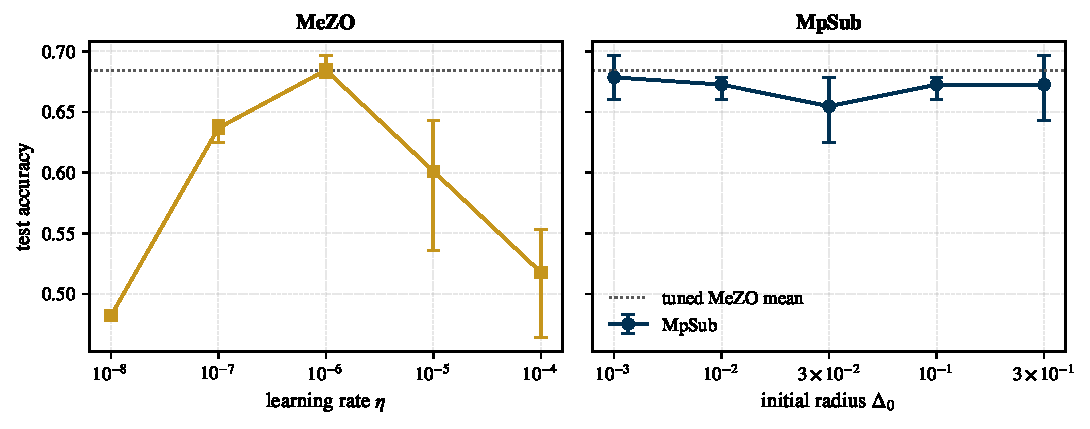
\includegraphics[width=0.98\textwidth]{fig_sensitivity.pdf}
\caption{Step-size sensitivity on OPT-125M under $8{,}400$ forward passes. Left: MeZO test accuracy across learning rates $\eta_{\mathrm{M}}$. Right: \texttt{MpSub} test accuracy across initial radii $\Delta_0$.}
\label{fig:sensitivity}
\end{figure}

MeZO is sensitive to its learning rate: varying $\eta_{\mathrm{M}}$ by one order of magnitude from $10^{-6}$ reduces test accuracy by $0.048$ at $10^{-7}$ and by $0.084$ at $10^{-5}$, requiring a grid search ($42{,}000$ forward passes on OPT-125M and $25{,}200$ on OPT-350M) to find an effective rate. Because $\eta_{\mathrm{M}}$ is held static throughout training, any mismatch between the chosen rate and the local curvature directly produces either premature stagnation or catastrophic divergence, necessitating an exhaustive sweep across multiple orders of magnitude ($10^{-8}$ to $10^{-4}$).

In contrast, \texttt{MpSub} shows little variation across the tested range: mean test accuracy remains between $0.655$ and $0.678$ across all five initial radii from $\Delta_0 = 10^{-3}$ to $3\times 10^{-1}$. This stability stems from the fundamentally different role of $\Delta_0$: it serves solely as an initial condition rather than an immutable step size. Under the geometric expansion rule \eqref{eq:radius_update_rule}, an overly conservative choice such as $\Delta_0 = 10^{-3}$ (two orders of magnitude below the default) doubles on successful steps and reaches the effective operating scale within $\lceil \log_2(10^2) \rceil \approx 7$ iterations, incurring negligible overhead over the 200-step budget. Conversely, excessively large initial radii ($\Delta_0 \gg 1$) are naturally avoided because $\Delta_k$ simultaneously sets the finite-difference perturbation in \eqref{eq:central_diff}, where oversized displacements degrade the accuracy of directional derivative estimates. Evaluating across the 300-fold span from $10^{-3}$ to $3\times 10^{-1}$ confirms that the default choice $\Delta_0 = 10^{-1}$ transfers reliably across model sizes without task-specific retuning.

\subsection{Effect of the subspace dimension}
\label{subsec:p_ablation}

Table~\ref{tab:p_ablation} examines the effect of varying the subspace dimension $p \in \{5, 10, \allowbreak 15, \allowbreak 20, \allowbreak 25, \allowbreak 30\}$ on OPT-125M over 100 iterations.

\begin{table}[htb]
\centering
\caption{Ablation on subspace dimension $p$ for OPT-125M (CommitmentBank, 100 steps, $\Delta_0 = 10^{-1}$, single seed). Forward passes per step equal $2p+2$; run times measured on an NVIDIA RTX 4060 Ti GPU.}
\label{tab:p_ablation}
\small
\begin{tabular}{ccccc}
\toprule
$p$ & Forward passes / step & Dev acc. & Test acc. & Time / step (s) \\
\midrule
5  & 12 & 0.70 & 0.643 & 3.0 \\
10 & 22 & 0.72 & 0.661 & 4.4 \\
15 & 32 & 0.74 & 0.661 & 6.0 \\
20 & 42 & 0.78 & 0.679 & 7.7 \\
25 & 52 & 0.78 & 0.679 & 8.7 \\
30 & 62 & 0.76 & 0.661 & 10.1 \\
\bottomrule
\end{tabular}
\end{table}

Across a fixed iteration horizon of 100 steps, increasing $p$ from 5 to 20 improves development accuracy from $0.70$ to $0.78$ and test accuracy from $0.643$ to $0.679$, in line with the richer directional derivative information captured by larger subspaces (Lemma~\ref{lem:capture}). Beyond $p = 20$, the per-step accuracy gain saturates while the forward-pass cost and wall-clock latency per step continue to grow linearly (from $3.0$ seconds at $p = 5$ to $10.1$ seconds at $p = 30$). Thus, $p = 20$ offers an effective operating point balancing subspace expressiveness against per-step computational overhead.

\section{Conclusion}
\label{sec:conclusion}

We proposed \texttt{MpSub}, which combines a random subspace with trust-region step-size control for derivative-free LLM fine-tuning. For smooth deterministic objectives, we proved that $\liminf_{k\to\infty} \|\nabla f(\bx_k)\|_2 = 0$ almost surely under Gaussian direction sampling and the safeguarded radius update, and established full convergence under the renewal property. On CommitmentBank, \texttt{MpSub} achieved results comparable to tuned MeZO on OPT-125M and OPT-350M under the same forward-pass budget, while using the same trust-region settings for both models.

Several questions remain open. The convergence analysis treats a fixed deterministic objective, whereas the LLM experiments resample the minibatch between iterations. Extending the analysis to changing minibatches is therefore the most direct theoretical next step. It would also be useful to study whether curvature information can be introduced into the subspace model without returning to the quadratic interpolation cost that motivated the linear model used here.

While this study evaluates classification on OPT-125M and OPT-350M, evaluating the method on larger models, broader benchmarks, and generative settings remains an important direction for future work. In addition, because the $2p$ directional evaluations within each iteration are mutually independent, parallel evaluation could substantially reduce wall-clock time. Finally, \texttt{MpSub} could be combined with parameter-efficient fine-tuning methods such as LoRA, where the trust-region mechanism would operate over a smaller parameter space.

\begin{acknowledgements}
The authors thank the developers of the MeZO and LOZO codebases, on which the experimental infrastructure builds.
\end{acknowledgements}

\section*{Declarations}
\paragraph{Funding} Not applicable.
\paragraph{Conflict of interest} The authors declare that they have no conflict of interest.
\paragraph{Data availability} The dataset analyzed during the current study is available in the SuperGLUE benchmark repository (\url{https://super.gluebenchmark.com}).

\bibliographystyle{spmpsci}
\bibliography{refs}

\end{document}
